\documentclass[a4paper,14pt]{article}

\usepackage[T2A]{fontenc}
\usepackage[utf8]{inputenc}
\usepackage[russian]{babel}
\usepackage[left=30mm, right=10mm,
            top=20mm, bottom=20mm,
            bindingoffset=0cm]{geometry}

\usepackage{graphicx}
\graphicspath{{.}}

\usepackage{hyperref}
\usepackage{indentfirst}

\title{Доклад на тему “Тепловые двигатели”}
\author{Чубий Савва}
\date{}

\begin{document}
    \textbf{\let\newpage\relax\maketitle}
    \thispagestyle{empty}
    \vspace{\fill}
    \tableofcontents
    \vspace{\fill}
    \pagebreak
    \setcounter{page}{1}

    %\large
    \pagebreak
    \section{Принцип работы и КПД тепловых двигателей}

        \underline{Тепловой двигатель} — это устройство, превращающее внутреннюю энергию топлива в механическую работу.

        Тепловой двигатель состоит из \textit{рабочего тела (обычно газа), нагревателя и холодильника (холоднее нагревателя).} Нагреватель греет рабочее тело, тело расширяется, совершая работу, потом отдает тепло холодильнику, для возврата в изначальное состояние.
        \begin{figure}[h]
            \center{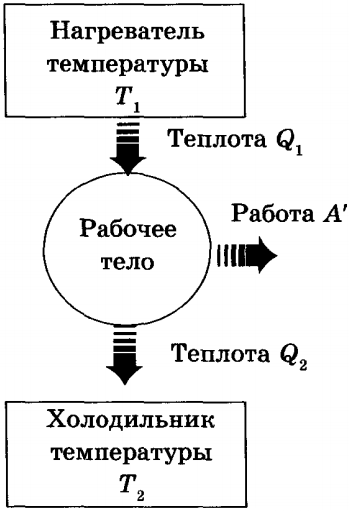
\includegraphics[height=6cm]{engine_scheme.png}}
            \caption{Схема теплового двигателя}
        \end{figure}

        \underline{КПД теплового двигателя} считают по формуле $\eta = \frac{A'}{Q_1}$, где $A'$ -- работа, совершенная двигателем, $Q_1$ -- количество теплоты, полученное телом от нагревателя.

    \section{Паровой поршневой двигатель}

        В этом двигателе рабочим телом является водяной пар, поступающий из котла, который толкает поршень.
        \begin{figure}[h]
            \center{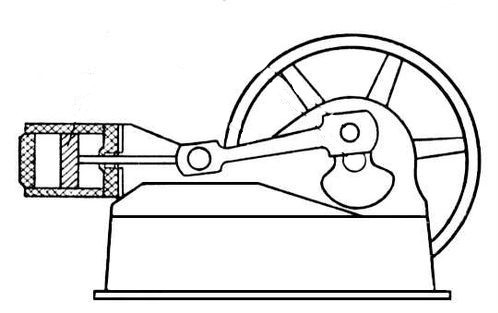
\includegraphics[height=6cm]{steam_machine.jpg}}
            \caption{Схема парового поршневого двигателя}
        \end{figure}

    \pagebreak
    \section{Бензиновый двигатель}
    \subsection{Бензиновый четырехтактный двигатель}

        Двигатель состоит из нескольких поршней. Каждый поршень состоит из \textit{двух клапанов (впускного и выпускного), камеры сгорания, поршня (вращающего вал) и других деталей.}

        Работа каждого цилиндра состоит из постоянно повторяющихся \textit{рабочих циклов}. Каждый цикл состоит из \textit{четырех тактов}:
        \begin{enumerate}
            \item Впуск\\
                Впускной клапан открывается (выпускной закрыт), поршень переходит из верхней мертвой точки (ВМТ) в нижнюю мертвую точку (НМТ), топливо заходит в камеру.
            \item Сжатие\\
                Клапан закрывается, поршень переходит в ВМТ, сжимая топливо.
            \item Рабочий ход (расширение)\\
                Топливо поджигается и расширяется, толкая поршень (он переходит в НМТ).
            \item Выпуск\\
                Открывается выпускной клапан, поршень движется к ВМТ, выталкивая сгоревшее топливо через клапан.
        \end{enumerate}
        \begin{figure}[h]
            \center{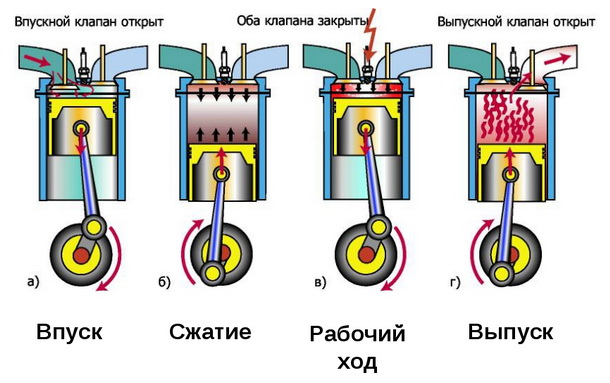
\includegraphics[height=6cm]{4-takta.jpg}}
            \caption{Схема работы бензинового четырехтактного двигателя}
        \end{figure}

        В один момент времени разные поршни находятся на разных тактах (это повышает плавность работы двигателя).
    \subsection{Бензиновый двухтактный двигатель}

        В отличие от четырехтактного, в цилиндрах двухтактного двигателя нет выпускного клапана (его роль играет поршень), а впускной клапан расположен в другом месте. Рабочий ход состоит из \textit{двух тактов}:
        \begin{enumerate}
            \item Сжатие\\
                Поршень движется из НМТ к ВМТ, закрывая впускное, а потом выпускное отверстия и сжимая топливо.
            \item Рабочий ход (расширение)\\
                Топливо поджигается и расширяется, толкая поршень (он переходит в НМТ).
        \end{enumerate}
        \begin{figure}[h]
            \center{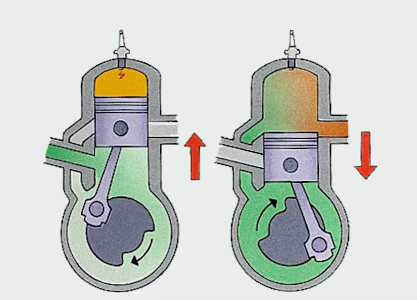
\includegraphics[height=6cm]{2-takta.png}}
            \caption{Схема работы бензинового двухтактного двигателя}
        \end{figure}
    \pagebreak
    \section{Дизельный двигатель}

    Дизельный двигатель сильно похож на четырехтактный бензиновый, но есть несколько отличий. В бензиновом воздух смешивают с топливом до подачи в цилиндр, потом поджигают во время такта расширения, в дизельном -- топливо (на том же такте)  впрыскивается в горячий воздух и самовоспламеняется (по этой причине в первом случае используется свеча зажигания, а во втором -- топливный инжектор).
    
        Бензиновые двигатели тише и меньше вибрируют. Это объясняется тем, что смесь бензина и воздуха горит плавнее, чем дизель.
    \section{Паровая турбина}
        
        Турбина состоит из \textit{диска с лопастями (лопатками), насаженного на вал, и сопла}. Водяной пар с большой температурой (около 600$^{\circ}C$) подается в сопло и там расширяется, увеличивая свою скорость. Струя пара подается на лопасти турбины, вращая диск и вал.

        Обычно турбины состоят из большого количества сопл и дисков.
        \begin{figure}[h]
            \center{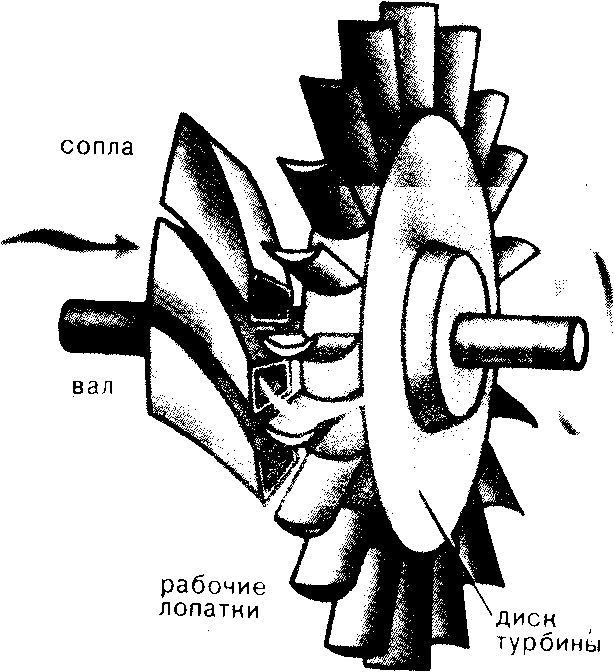
\includegraphics[height=6cm]{steam_turbine.png}}
            \caption{Схема паровой турбины}
        \end{figure}
        
    \pagebreak
    \section{ГТД, ТВД и ТРД}
    \subsection{Газотурбинный двигатель(ГТД)}
        Простейшая модель газотурбинного двигателя состоит из \textit{вала, на котором закреплены два диска с лопатками (диск компрессора и диск турбины), между которыми расположена камера сгорания.}

        Компрессор сжимает воздух и подает его в камеру сгорания. Сжатый воздух смешивается с топливом и поджигается, расширяясь, раскручивает диск турбины, который раскручивает вал и диск компрессора.
        \begin{figure}[h]
            \center{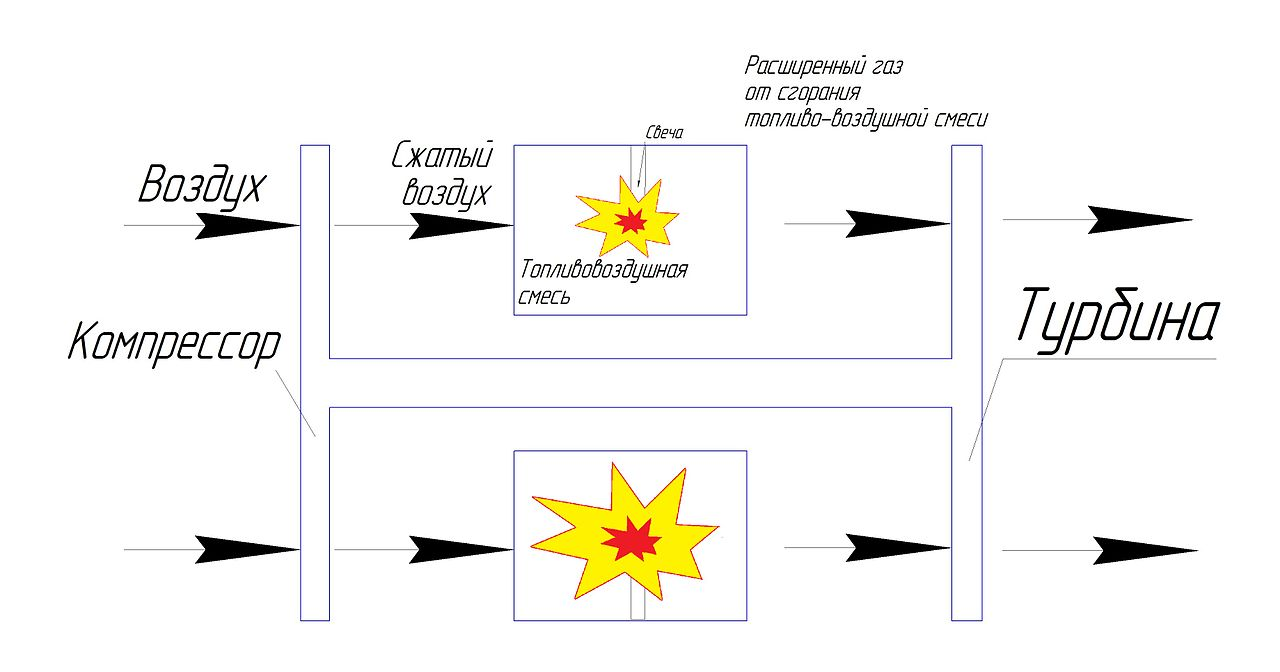
\includegraphics[height=6cm]{gas_turb.jpg}}
            \caption{Схема модели газотурбинного двигателя}
        \end{figure}
    \subsection{Турбореактивный двигатель(ТРД)}
        ТРД очень похож на ГТД, но в ГТД полезная мощность снимается с вала, а в ТРД полезная мощность -- это реактивная струя (для получения струи в ТРД имеется сопло).
        \begin{figure}[h]
            \center{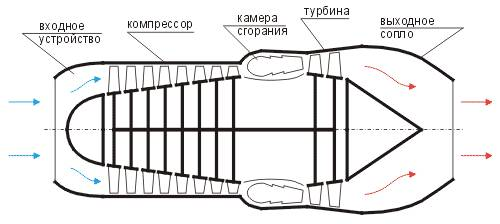
\includegraphics[height=6cm]{TRD.jpg}}
            \caption{Схема модели турбореактивного двигателя}
        \end{figure}
    \subsection{Турбовентиляторный двигатель(ТВД)}
        ТВД и ТРД также очень похожи, но в ТВД на входе расположен большой вентилятор. Всасываемый вентилятором воздух разделяется на два потока (один, как и в ТРД, идет внутреннее ядро двигателя (примерно 15\% всасываемого воздуха), другой -- обтекает ядро снаружи и попадает в сужающую камеру, потом выбрасывается наружу). Обтекающий ядро воздух выдает, примерно, 80\% мощности.
        \begin{figure}[h]
            \center{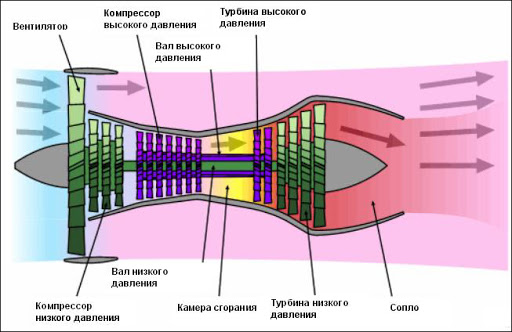
\includegraphics[height=6cm]{TVD.jpg}}
            \caption{Схема модели турбовентиляторного двигателя}
        \end{figure}
    \pagebreak
    \section{Ракетные двигатели}
        Задача ракетного двигателя -- выбрасывать большую массу с большой скоростью, тогда по третьему закону Ньютона ракете будет сообщаться импульс, за счет которого она будет лететь.

    \subsection{Твердотопливный ракетный двигатель}
        Топливо должно быстро гореть, но не взрываться. По этой причине оружейный порох не подойдет, но если изменить пропорции ингредиентов, то получится подходящая смесь.

        Принцип работы прост: топливо размещают определенным образом и поджигают.

        Твердотопливные двигатели обладают важными \textit{преимуществами}:
        \begin{itemize}
            \item простота
            \item низкая стоимость
            \item безопасность
        \end{itemize}
        Но есть и \textit{недостатки}:
        \begin{itemize}
            \item невозможно контролировать тягу
            \item после зажигания двигатель нельзя отключить
        \end{itemize}

        Из-за этих недостатков двигатели можно использовать только для непродолжительных задач или систем ускорения.
        \begin{figure}[h]
            \center{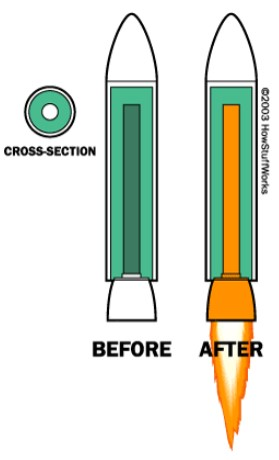
\includegraphics[height=6cm]{hard_rocket.jpg}}
            \caption{Схема твердотопливного ракетного двигателя до и после зажигания (зеленым обозначено топливо)}
        \end{figure}
    \subsection{Жидкотопливный ракетный двигатель}
        Двигатель состоит из \textit{бака с топливом, бака с окислителем, насосов, клапанов, камеры сгорания и сопла.}

        В камере сгорания смешиваются и сгорают смесь топлива и окислителя, продукты горения поступают в сопло, которое ещё больше увеличивает их скорость (от до- до сверхзвуковой), затем выбрасываются наружу.
    \begin{figure}[h]
        \center{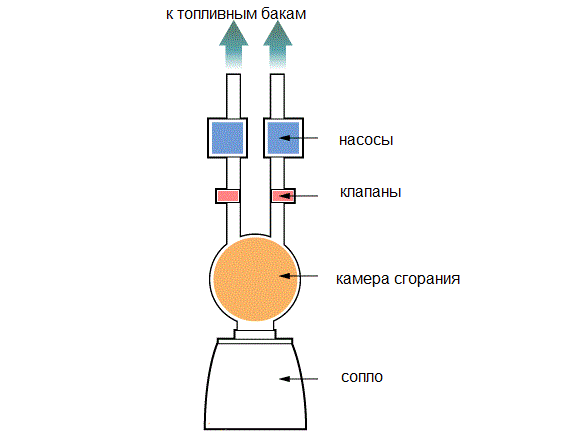
\includegraphics[height=6cm]{fluid_rocket.png}}
        \caption{Схема жидкотопливного ракетного двигателя}
    \end{figure}

    \section{Двигатель Стирлинга}
        Принцип работы заключается в том, что рабочее тело, находящееся в закрытом цилиндре поочередно перегоняется \textit{вытеснителем} от источника тепла к источнику холода.
        \textit{Маховик} позволяет двигателю не останавливаться в мертвых точках.
        \begin{figure}[h]
            \center{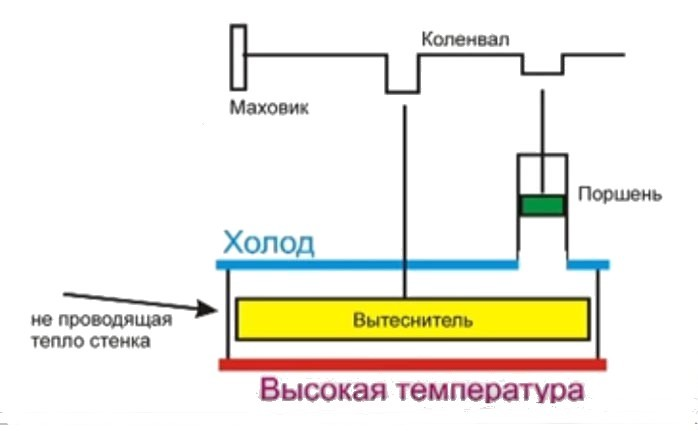
\includegraphics[height=5cm]{stirling.jpg}}
            \caption{Схема двигателя Стирлинга}
        \end{figure}

    \pagebreak
    \section{Список источников}
    \begin{itemize}
        \item Н.С.Пурышева, Н.Е.Важеевская, Физика, 8 класс
        \item \url{https://www.calc.ru/Teplovoy-Dvigatel-Printsip-Deystviya-Teplovykh-Dvigateley.html}
        \item \url{https://www.booksite.ru/fulltext/1/001/008/087/088.htm}
        \item \url{https://www.youtube.com/watch?v=yZ8w_WEMbEU}
        \item \url{https://www.studiplom.ru/Technology-DVS/2-x_DVS.html}
        \item \url{https://www.youtube.com/watch?v=Ob5M0EVh9lo}
        \item \url{https://www.youtube.com/watch?v=4JJsIuqZbbA}
        \item \url{https://hi-news.ru/technology/kak-rabotayut-raketnye-dvigateli.html}
        \item https://ru.wikipedia.org/wiki/Газотурбинный\_двигатель%\url{https://ru.wikipedia.org/wiki/%D0%93%D0%B0%D0%B7%D0%BE%D1%82%D1%83%D1%80%D0%B1%D0%B8%D0%BD%D0%BD%D1%8B%D0%B9_%D0%B4%D0%B2%D0%B8%D0%B3%D0%B0%D1%82%D0%B5%D0%BB%D1%8C}
        \item \url{https://www.youtube.com/watch?v=qrNV_JQawJw}
        \item \url{https://www.youtube.com/watch?v=XMR9dfm0EoI}
    \end{itemize}
\end{document}
